\documentclass{article}

\usepackage[utf8]{inputenc}
\usepackage[spanish]{babel}
\usepackage{amsthm}
\usepackage{nccmath}
\usepackage{enumitem}
\usepackage{graphicx}
\usepackage{verbatim}
\usepackage{algpseudocode}

\theoremstyle{plain}
\newtheorem{proposicion}{Proposición}

\theoremstyle{definition}
\newtheorem{definition}{Definición}[section]
\newtheorem{example}{Ejemplo}[section]

\title{Teoría de Autómatas y Lenguajes Formales\\[.4\baselineskip]Práctica 3.}
\author{Alejandro Rodríguez Moreno}
\date{Diciembre 2022}

\begin{document}

\maketitle

\section{Descripción de los autómatas}

Un autómata finito determinista(AFD) es una quíntupla(K, $\sum$, $\delta$, s, F).

\vspace{6mm}

- K es un conjunto finito no vacío de estados.

\vspace{4mm}

- $\sum$ es un alfabeto.

\vspace{4mm}

- s es el estado inicial el cual debe de encontrarse tal que s $\in$ K.

\vspace{4mm}

- F es el conjunto de estados finales.

\vspace{4mm}

- $\delta$ es una función de transición.

\newpage
\section{AFD que reconozca dicho lenguaje}
Ejemplo de un AFD generado con JFLAP y cadenas, que reconoce el lenguaje previamente mencionado.

\begin{center} 
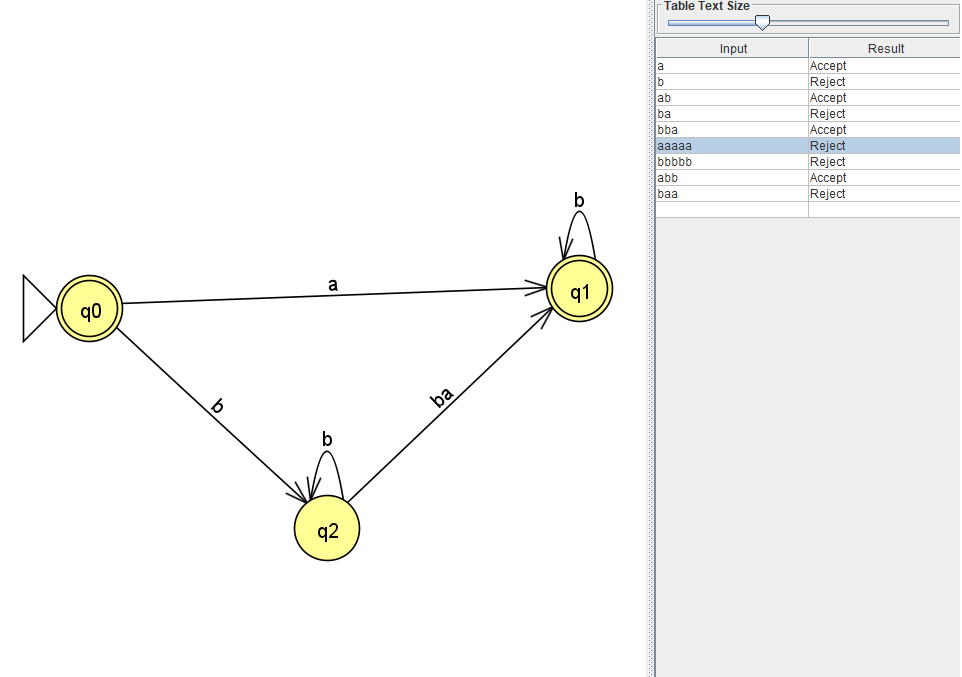
\includegraphics[width=13cm, height=9cm]{P2_Automata.png}
\end{center}

\section{JSON del automata ejemplo}

\begin{verbatim}
    {
    "name" : "a",
    "representation":{
    "K" : ["q0", "q1", "q2"],
     "A" : ["a","b"],
     "s" : "q0",
     "F" : ["q1"],
     "t" : [["q0", "a", "q1"],
            ["q0", "b", "q2"],
            ["q1", "b", "q1"],
            ["q2", "b", "q2"],
            ["q2", "ba", "q1"]]
}  }
            
      }
\end{verbatim}


\end{document}

